\section{Results}
This section will display the results of this research. It presents and discusses the Article Count, the Polarity of the text for specific parties, the Subjectivity of the text for specific parties etc. To generate valid conclusions, both an exclusive and normal data set have been generated. The exclusive data set is generated using articles which are only about a specific party, while the normal data set contains articles which can feature multiple parties. Based on the case, a choice will be made whether to use the exclusive or the normal data set to draw a conclusion.

\subsection{General}
The number of the articles in the data set of {\it de Volkskrant} is 491 852. The mean values and the standard deviation of the subjectivity scores for text and description are calculated. \\
\begin{table}[h]
  \begin{tabular}{ l | c | c }
  &Mean&Standard deviation\\
  \hline
  Text polarity&0.039&0.1522\\
  Text subjectivity&0.5065&0.1696\\
  Description polarity&0.0323&0.2319\\
  Description subjectivity&0.3233&0.3250\\
  \end{tabular}
  \caption{Polarity and subjectivity scores for {\it de Volkskrant}}
  \label{tab:general}
\end{table}
The results show that polarity and subjectivity scores vary much more for the description than for the text. However, it makes the text more suitable for comparing the sentiment score of the political party related articles to the overall scores in the newspaper.

The political related research starts with getting the relative article count per political party in {\it de Volkskrant}. The political parties included in this research are only the members of the current parliament of the Netherlands. The relative percentage of articles written per political party is shown below in Figure \ref{fig:article_count_exclusive}. \\
    \begin{figure}[ht]
        \centering
        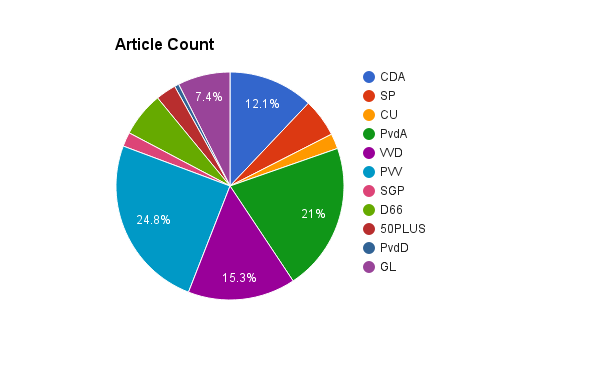
\includegraphics[scale=0.43]{Graphs/article_count_exclusive}
        \caption{Relative article count per political party}
        \label{fig:article_count_exclusive}
    \end{figure}
It can be concluded that {\it de Volkskrant} has written the most politically motivated articles about the PVV and the PvdA. Parties which are not much talked about are PvdD and SGP. The counts have been generated from the exclusive data set to ensure that one single article doesn't count for multiple parties. \\
\subsection{Political Articles}
\begin{table}[h]
  \begin{tabular}{ l | c | c | c }
  Party&Article Count&Polarity&Subjectivity\\
  \hline
CDA&3186&0.0341&0.5157 \\
SP&1822&0.0314&0.5143 \\
CU&1264&0.0314&0.5077 \\
PvdA&3925&0.0321&0.5157 \\
VVD&4051&0.0327&0.5169 \\
PVV&3175&0.0196&0.5213 \\
SGP&823&0.0335&0.5058 \\
D66&2236&0.0346&0.5116 \\
50PLUS&352&0.0115&0.4867 \\
PvdD&86&0.0109&0.4989 \\
GL&1740&0.0314&0.516
  \end{tabular}
  \caption{Polarity and subjectivity scores in text per party}
  \label{tab:party_scores}
\end{table}

The research continues with counting the number of articles per political party with their sentiment scores. The result shows if the data is enough to yield statistically significant results.

Next step is to look into the overall tone for the political parties from the point of view of the newspaper using articles posted by the {\it de Volkskrant Redactie}.
    \begin{figure}[ht]
        \centering
        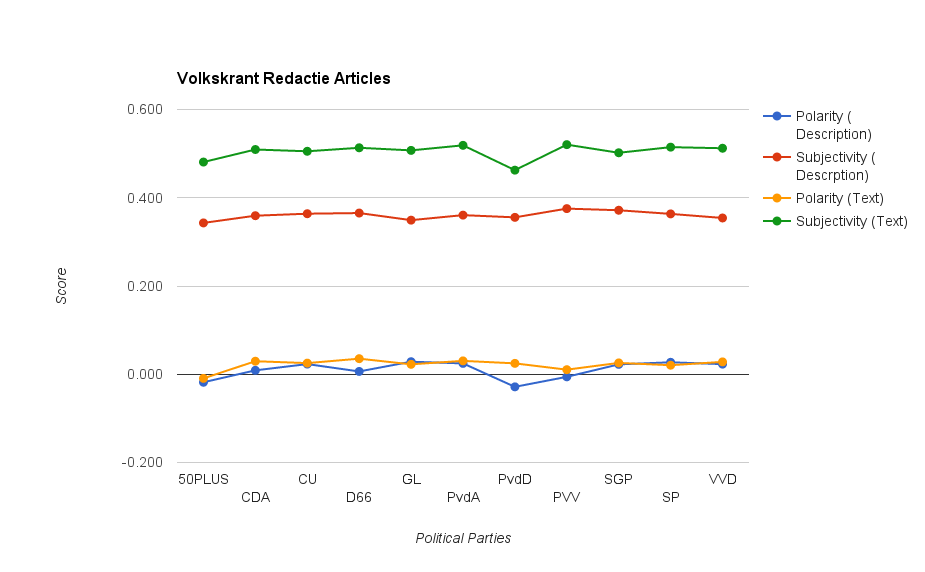
\includegraphics[scale=0.28]{Graphs/VolkskrantRedactieV2}
        \caption{Polarity and subjectivity of {\it de Volkskrant Redactie}}
        \label{fig:volkskrantr}
    \end{figure}
    \\
It is shown in Figure \ref{fig:volkskrantr} that {\it de Volkskrant Redactie} is neutral to slightly positive to most of the parties. One can see that the PvdD is the least liked out of the parties. The results also display that the text is much more subjective than the description.

The research continues with observing the change of polarity in articles over the years. The political parties selected for graph have enough articles for statistically significant results. Figure \ref{fig:polarity} shows how the polarity of the articles about PvdA, PVV and VVD has changed in the period from 2010 to 2016.
    \begin{figure}[ht]
        \centering
        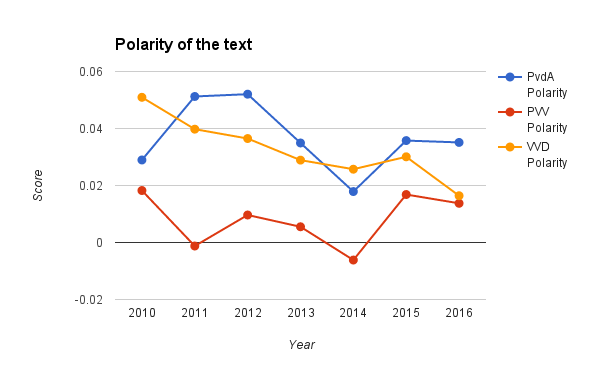
\includegraphics[scale=0.40]{Graphs/Polarity}
        \caption{Polarity of articles about PvdA, PVV and VVD over time}
        \label{fig:polarity}
    \end{figure}
    \\
From the Figure \ref{fig:polarity} we can see that the polarity of the VVD has moved from the positive towards the neutral. The PvdA is back on the same polarity as it was in 2010. The PVV has been shifting from slightly positive to slightly negative and back. 

Furthermore, a set of {\it Z}-tests have been performed for the parties shown in Figure \ref{fig:polarity}. Tested is whether the polarity score of articles about specific parties from the Volskrant is significantly different compared with the average polarity score of the articles in the 'Politiek' section. 
The average and standard deviation of polarity scores of the text of articles in the 'Politiek' section are 0.0300 and 0.1331, respectively. \\

The PvdA has a mean text polarity score of 0.0381. The resulting z-score is 6.7961. The corresponding tow-tailed p-value is smaller than 0.0001. Therefore the two samples are significantly different.

The PVV has a mean text polarity score of 0.0070. The resulting z-score is -19.2975. The corresponding tow-tailed p-value is smaller than 0.0001. Therefore the two samples are significantly different.

The VVD has a mean text polarity score of 0.0318. The resulting z-score is 1.5102. The corresponding tow-tailed p-value is 0.131. Therefore the two samples are not significantly different. \\

The above results show that {\it de Volkskrant} is not significantly biased towards the VVD, a right-wing party, while it is negative towards the PVV, which is a centrist party. Furthermore, {\it de Volkskrant} is positive toward the PvdA, which is a left-wing party. There can be concluded that {\it de Volkskrant} is left motivated. \\

    \begin{figure}[ht]
        \centering
        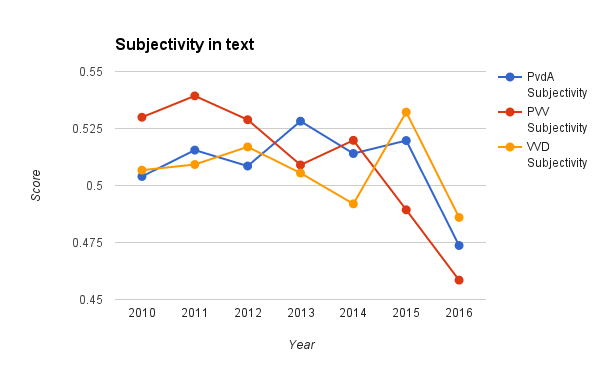
\includegraphics[scale=0.40]{Graphs/Subjectivity}
        \caption{Subjectivity of articles written about three political parties over the year}
        \label{fig:subjectivity}
    \end{figure}
    \\
For the subjectivity as shown in Figure \ref{fig:subjectivity} can be seen that all of the parties had subjectivity in the articles written about them. However there is a decline in subjectivity towards 2016. \\

Also, a set of {\it Z}-tests have been performed for the parties shown in Figure \ref{fig:subjectivity}. Tested is whether the subjectivity score of articles about specific parties from the Volskrant is significantly different compared with the average subjectivity score of the articles in the 'Politiek' section. 
The average and standard deviation of subjectivity scores of the text of articles in the 'Politiek' section are 0.5097 and 0.1334, respectively. \\

The PvdA has a mean subjectivity score of 0.5118. The resulting z-score is 1.758. The corresponding tow-tailed p-value is 0.0788. Therefore the two samples are not significantly different.

The PVV has a mean subjectivity score of 0.5237. The resulting z-score is 11.7199. The corresponding tow-tailed p-value is smaller than 0.0001. Therefore the two samples are significantly different.

The VVD has a mean subjectivity score of 0.5100. The resulting z-score is 0.2511. The corresponding tow-tailed p-value is 0.8017. Therefore the two samples are not significantly different. \\

The above results show that {\it de Volkskrant} only is significantly subjective in articles about the PVV. This strengthens the obtained result that {\it de Volkskrant} is biased towards the PVV.

\subsection{Validation}
The results have been validated by looking at different data sources. In this master thesis\cite{Xthesis:volkskrant} the political alignment of {\it de Volkskrant} is described as "centre-left". This means that the Volkskrant is generally in favour of the PvdA and D66. However, the political tone in {\it de Volkskrant} articles is not always clear, as the articles are generally not pronounced. {\it De Volkskrant} gives little information about the true nature of the newspaper. The AD\cite{ad_voters} gives an overview of the political preference of the readers of the Dutch press. The political preference in general of {\it de Volkskrant} readers is PvdA and D66. The results show that the polarity of the main text of the articles from the editorial office on the PvdA and D66 is relatively positive in comparison with the other political parties. \\